\xchapter{Fundamentação teórica}{}
\label{fundamentacao}

Este capítulo apresenta conceitos necessários para a compreensão do trabalho
acerca de ecossistema de software (Seção \ref{sec:ecos}),
ecossistemas de software acadêmico (Seção \ref{sec:ecossa}),
modelo de desenvolvimento de software acadêmico (Seção \ref{sec:modelosa}),
software de análise estática (Seção \ref{analise-estatica}),
sustentabilidade (Seção \ref{sec:sustentabilidade}) e modelo de estágios
para ciclo de vida do software (Seção \ref{sec:ciclo}).

\section{Ecossistema de software}

Ecossistema de software é definido, segundo \citeonline{manikas2013software},
como a interação entre diversos atores numa plataforma tecnológica comum,
resultando em novas soluções de software ou novos serviços. Atores do
ecossistema, motivados por um conjunto de interesses, conectam-se entre si e ao
próprio sistema numa relação simbiótica, fazendo a plataforma tecnológica
evoluir enquanto permite o envolvimento e contribuição de novos e diferentes
atores \cite{manikas2013software}.

Nesta relação, os atores são beneficiados de formas diferentes a depender da
natureza do ecossistema. Num ambiente comercial, por exemplo, os atores são
beneficiados diretamente através de receita financeira (salário, prêmios, etc),
enquanto num sistema não-comercial os atores estão motivados por questões
não-monetárias, como fama, reconhecimento, ideologia, etc
\cite{manikas2013software}.

De modo geral, em ecossistemas de software, os benefícios recebidos pelos
atores e proporcionados pelo ecossistema, aumentam com o passar do tempo por
meio de uma relação de benefício mútuo.  Este modelo geral de funcionamento, no
entanto, pode variar a depender do contexto em que se insere o ecossistema,
especialmente no relacionamento entre os atores que pode variar entre
mutualismo, parasitismo, antagonismo e competição, etc
\cite{manikas2013software}.

\section{Ecossistema de software acadêmico}

O ecossistema de software acadêmico possui a particularidade de se relacionar
com o sistema econômico de reputação científica, especialmente com o seu modelo
de publicações, influenciando e sendo influenciado diretamente pelo impacto de
suas publicações \cite{howison2015understanding}.

Neste cenário, interessado em compreender as relações neste ecossistema,
\citeonline{howison2015understanding} criou um framework para pensar e refletir
sobre o processo de produção de software no meio científico, e identificou quatro
papéis básicos envolvidos no ecossistema de software acadêmico: 
(1) cientistas usuários finais, (2) produtores e distribuidores de software, (3)
administradores de infraestrutura e (4) pesquisadores preocupados com o
funcionamento do ecossistema como um todo.

\subsection{Cientistas usuários finais}

Cientistas ocupam papel chave no ecossistema de software acadêmico.  Em seus
processos de investigação e experimentação, fazem uso crescente de software
para coleta, gerenciamento, transformação, análise, modelagem e visualização de
dados. Além da preocupação com qualidade e usabilidade, estes cientistas estão
também preocupados com a disponibilidade e com a capacidade do software em
continuar sendo útil \cite{howison2015understanding}.

Finalmente, cientistas estão interessados também em saber o que outros
cientistas estão usando em suas pesquisas. A alta adoção de um software, além
de ser um bom indicador de qualidade, mantém os cientistas mais livres e com
maior foco em suas próprias pesquisas, uma vez que podem encontrar ajuda entre
os seus pares para resolver questões sobre o uso do software
\cite{howison2015understanding}.

%e de podendo ser utilizado em conjunto com outras
%soluções de software.

%garantir que o grupo de pesquisa, estudantes e colaboradores consigam 
% simplifica também o trabalho dos
%revisores pois encontrarão as mesmas facilidades no uso.

\subsection{Produtor e distribuidor de software acadêmico}

O papel de produtor e distribuidor de software costuma ser desempenhado por
equipes colaborando entre sí, geralmente compostas por cientistas da computação
e cientistas do domínio onde a pesquisa se insere.
Geralmente, o cientista da computação é o responsável por implementar os
algoritmos, métodos ou resultados gerados pelo estudo
\cite{howison2015understanding}.

Um desafio comum enfrentado neste papel é conseguir abstrair os problemas e
implementar soluções abrangentes em software.
Muitas vezes, o software criado fica confinado em seu laboratório ou grupo, mas
eventualmente é compartilhado e amplamente adotado, tornando o cientista autor
do software e da pesquisa parte do ecossistema \cite{howison2015understanding}.

Entre as inúmeras preocupações do produtor e distribuidor de software, podemos
destacar a preocupação acerca de como o software contribui para as
investigações científicas que outros pesquisadores estão realizando.
Alguns projetos são gerenciados no estilo de código aberto, e têm atraído com
sucesso contribuições de muitos cientistas, incluindo contribuidores que tem
fazem pequenas, porém substanciais contribuições
\cite{howison2015understanding}.

\subsection{Provedor de infraestrutura}

O provedor de infraestrutura é aquele que provê cojuntos de software aos
cientistas usuários finais. Este conjunto pode estar disponível em forma de
download para que seja utilizado em computadores pessoais ou pode estar
disponível em forma de serviços, como por exemplo, ciberinfraestrutura
\cite{council2007cyberinfrastructure, stewart2010cyberinfrastructure} de
software.
%ciberinfraestrutura de software hospedados em centros de supercomputação
%usando provedores de computação em nuvem.

Do ponto de vista do ecossistema, os dois tipos de distribuição implicam nas
mesmas preocupações e questões: quem usa o software, qual versão é utilizada, 
qual a frequencia de atualização, entre outras \cite{howison2015understanding}.
% preocupações relacionadas à distribuição e uso.

\subsection{Pesquisador}

Este último papel, chamado de pesquisador num sentido amplo, refere-se a
qualquer pessoa preocupada com o funcionamento do ecossistema e com a sua
contribuição para a Ciência. O papel de pesquisador costuma ser desempenhado
por agências de fomento ou por cientistas preocupados com o seu trabalho
individual e com o impacto em seu campo de pesquisa
\cite{howison2015understanding}.

As preocupações incluem questões sobre a operação do ecossistema
como um sistema que consome recursos (tempo, dinheiro e atenção) e afeta a
conduta da ciência, tanto no geral como em campos específicos, 
e sobre a compreensão do comportamento desse sistema e de 
como pode ser influenciado \cite{howison2015understanding}.

\section{Modelo de desenvolvimento de software acadêmico}

% recurso, uso e impacto

Cada ator desempenha um papel importante na estabilidade e sustentabilidade do
ecossistema \cite{dhungana2010software}. Assim como nos ecossistemas naturais,
o ecossistema de software necessita de fornecimento constante de energia, seja
na forma de novos desenvolvimentos ou na forma de ações de manutenção
\cite{dhungana2010software}.

Os atores participam dentro de seus próprios interesses, mas sempre causando
impacto no sistema como um todo \cite{manikas2013software}.
Cientistas usuários finais usam software acadêmico (direta ou indiretamente)
para fazer Ciência, resultando em impacto científico. Tal impacto científico
justifica novos investimentos, fazendo o ecossistema crescer
\cite{howison2015understanding}.

\begin{figure}[h]
  \center
  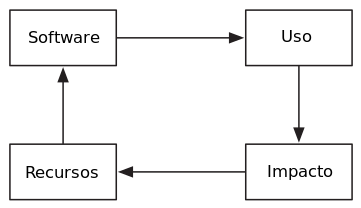
\includegraphics[scale=0.5]{imagens/process-model-scientific-software-dia.png}
  \caption{Um modelo de processo de software na Ciência~\cite{howison2015understanding}}
  \label{process-model-scientific-software}
\end{figure}

A Figura \ref{process-model-scientific-software} apresenta um modelo de
desenvolvimento de software acadêmico, explicitando as relações entre os
elementos \textit{software}, \textit{recursos}, \textit{uso} e
\textit{impactos}, detalhados a seguir.

\subsection{Software acadêmico}

Software acadêmico ({\it academic software}) é todo software usado para
coletar, processar ou analisar resultados de pesquisas com intenção de
publicação na literatura acadêmica (periódicos, revistas, conferências,
monografias, livros ou teses), incluindo desde protótipos escritos pelos
próprios cientistas, a produtos completos desenvolvidos profissionalmente
\cite{allen2017engineering}.

Podem ser projetos de software desenvolvidos num modelo de {\bf Software como
serviço de suporte} ({\it Software as Supporting Service}), sobrevivendo
totalmente à parte do sistema de reputação acadêmica, ou no modelo de {\bf
Software para crédito acadêmico} ({\it Software for academic credit}), estando
seu desenvolvimento intrinsecamente associado ao sistema de reputação acadêmica
\cite{howison2011scientific}.

No segundo caso, Software para crédito acadêmico, a relação com o sistema de
reputação acadêmica pode ainda variar entre motivações distintas resultando em
(1) Software Incidental ({\it Incidental software})
feito puramente para apoiar e facilitar pesquisas,
(2) Prática de software paralela ({\it A parallel software practice})
feito com objetivo de ser utilizado por outros pesquisadores, ou
(3) Um subcampo de software ({\it A Software Subfield}),
onde o próprio software é considerado uma contribuição primária para a Ciência
\cite{howison2011scientific}.

%reputação direta pelo trabalho com o software.
%geralmente publicado em artigo de ferramenta em paralelo aos artigos sobre 
%a pesquisa principal sobre o domínio sendo estudado,

%Garante sua sobreviência independente do sistema de reputação acadêmica,
%geralmente software comercial,
%feito por desenvolvedores de software contratados,
%não costuma receber menção na literatura acadêmica.


  %Software for academic credit
  %\item [Software para crédito acadêmico]

%Está intrinsecamente associado ao sistema de reputação acadêmico,
%tendo como principal incentivo o crédito acadêmico, sendo desenvolvido
%como um Software Incidental ({\it Incidental software})
%feito puramente para apoiar e facilitar a pesquisa,
%como Uma Prática de Software Paralela ({\it A parallel software practice})
%feito com objetivo de ser utilizado por outros pesquisadores,
%geralmente publicado em artigo de ferramenta em paralelo aos artigos sobre 
%a pesquisa principal sobre o domínio sendo estudado,
%como Um Subcampo de Software ({\it A Software Subfield}),
%onde o software é considerado uma contribuição primária para a ciência,
%reputação direta pelo trabalho com o software.

%Incidental software
%typically written by individuals and not made available for
%others to use, at least not in any formal or on-going way.
%
%  %
%  [Uma prática de software paralela]
%        (scientific needed enhanced by publishing 'software papers' alongside domain research)
%
%  %
%  [Um subcampo de software]
%        (reputação direta pelo trabalho do software);
%o segundo sistema de produção que está associado ao crédito acadêmico
%publicações sobre software costuma ser visto como contribuição primária

  %Hybrids
%  \item [Híbridos]
%        licença-dual e 'software work' dentro de grandes colaborações (software como uma contribuição científica direta)
%
%\end{description}

%Software acadêmico também é referenciado na literatura acadêmica como
%{\it research tool} \cite{Portillo12},
%{\it research-originated software} \cite{Kon2011},
%{\it research software} \cite{hettrick2014uk} ou
%{\it scientific software} \cite{segal2008developing}.
%%esses artefatos tem sido estudados dos mais variados pontos
%%de vista, desde de sua qualidade interna, até o impacto que
%%causam no meio científico.

% Proprietary versus public domain licensing of software and research products
% este paper mostra que usar GPL em software traz vantagens e fala dos problemas em nao disponibilizar software academico

%Entre as inúmeras funções desempenhadas pelo software acadêmico em suas
%pesquisas, identificam-se motivações distintas para a sua criação,
%seis modelos de produção de software na ciência que abstraem uma série de
%características sobre como são criados, mantidos e compartilhados,
%estes modelos são caracterizados especialmente pelos incentivos e
%recompensas disponíveis aos seus atores e estão associados a um conjunto de
%práticas de engenharia de software \cite{howison2011scientific}.

\subsection{Recursos}

Os recursos investidos na produção de software acadêmico vêm de diversas
fontes, incluindo ganhos monetários diretos, recursos alocados em projetos, e
colaboração entre laboratórios de pesquisa \cite{howison2015understanding}.
Grande parte dos recursos vem do ``tempo livre'' dos pesquisadores em busca de
soluções para suas pesquisas e perpassa por financiamentos diversos obtidos na
carreira individual do cientista, prêmios recebidos, etc
\cite{howison2015understanding}.

Independente da origem dos recursos, grande parte do desenvolvimento de
software acadêmico é realizado pelos próprios cientistas \cite{hettrick2014uk,
momcheva2015software}.
Esta tendência tem sido interpretada como um reflexo do conhecimento sobre
domínio da pesquisa muitas vezes necessário ao desenvolvedor deste software
\cite{segal2008developing}.

No caso da pesquisa em Engenharia de Software, este conhecimento teórico sobre
o domínio se confunde, muitas vezes, com a própria prática de desenvolvimento.

\subsection{Uso}

% ... software é distribuido, utilizado e dá suporte à ciencia, gerando impacto ...

Metade dos pesquisadores de todas as áreas da Ciência fazem uso intenso de
software acadêmico, desde grupos trabalhando exclusivamente com problemas
computacionais até grupos em laboratórios tradicionais ou em campo
\cite{wilson2014best}.

Este uso é mencionado em suas pesquisas, por meio de citação formal ou informal
\cite{smith2016software}.
Estas menções são parte do sistema econômico de reputação científica e causam
impacto científico direto tanto na publicação quanto no ecossistema de software
acadêmico\cite{katz2014transitive}.

Este impacto direto geralmente justifica o investimentos de novos recursos no
ecossistema, seja para fins de planejamento, como retrospectiva para avaliar
investimentos já realizados ou para promover evolução do software acadêmico
\cite{howison2015understanding}.

\subsection{Impacto científico}

Ao longo da história, a citação formal tem sido utilizada para garantir
autenticidade e autoridade, ao invés de crédito e reconhecimento
\cite{katz2014transitive}.
Na história ocidental, a citação surge no final do século XVI e, no início do
século XVIII surgem o sistema legal por trás do sistema de citações e a lei de
``copyright'' para garantir os direitos dos autores \cite{katz2014transitive}.

Apesar do grande uso para garantir autenticidade e autoridade, o sistema de
citações e a informação sobre a autoria das publicações tem sido realmente
utilizado para avaliações importantes dentro do corpo científico
\cite{katz2014transitive}.
Por exemplo, ``backward citing'' tem sido utilizado para se certificar quem de
fato contribuiiu para um certo avanço ou descoberta, e ``forward citing'' tem
sido usada em casos onde se quer entender como uma idéia foi usada após o seu
surgimento ou publicação \cite{katz2014transitive}.

%Tradicionalmente, um autor cita um artigo anterior adicionando uma referência 
%ao autor, título, local de publicação, etc.

Conhecimento novo é claramente construído a partir do conhecimento passado e o
sistema de citações formais tem promovido avanços significativos
\cite{katz2014transitive}.
No entanto, esse conceito não tem funcionado tão bem para produtos digitais
como o software, que muitas vezes depende de outro software, fragmentos de
código, e algoritmos \cite{katz2014transitive}.

Este debate ocorre há bastante tempo entre as diversas áreas da bibliometria,
cienciometria, altmetria e áreas similares \cite{gouveia2013altmetria}.
Por exemplo, o fator de impacto, proposto na década de 90
\cite{reuters2017history}, apesar de contribuir para a Ciência, por
vezes é utilizado da forma errada e mostra as deficiências de lidar bem com
produtos digitais gerados durante pesquisas \cite{katz2014transitive}.

%%% PAREI AQUI %%%

%%%%%%%%%%%%%%%%%%%%%%%%%%%%%%%%%%%%%%%%%%%%%%%%%%%%%%%%%%%%%%%%%%%%%

%Cita um mapeamento feito sobre estudos que criam ferramentas para apoio a
%revisão sistemática no domínio de SE, 14 estudos foram selecionados, ao final
%apenas 8 tinham proposta de ferramentas, ao final conclui que as ferramentas
%encontradas estão em estado inicial de desenvolvimento \cite{marshall2013tools}.

%Cita um mapeamento sistemático com objetivo de encontrar ferramentas de
%comunicação e coordenação para suporte a times altamente distribuidos
%gograficamente, encontrou 132 ferramentas, para uso em projetos de software
%global. A maioria destas ferramentas foram desenvolvidas em centros de
%pesquisas, e apenas uma pequena porcentagem (18.9\%) foram testados fora do
%seu contexto onde foi desenvolvido \cite{Portillo12}.

%Computer systems research spans sub-disciplines that in-
%clude embedded and real-time systems, compilers, network-
%ing, and operating systems. Our contention is that a number
%of structural factors inhibit quality research. We highlight
%some of the factors we have encountered in our work and ob-
%served in published papers and propose solutions that could
%both increase the productivity of researchers and the quality
%of their output \cite{Vitek2011}.

%Além da aplicação, estes softwares variam também no papel que ocupam em suas
%pesquisas, alguns fazem parte dos resultados da pesquisa, como por exemplo,
%propostas de novos algoritmos ou técnicas de produção, outros são utilizados
%como parte do método de pesquisa, como coleta ou análise de dados, sendo que
%estes papeis não são excludentes.
%
%estes costumam ser citados pelos seus autores como uma das contribuições do
%estudo, seja principal ou secundária, 
%Esses softwares podem, de fato, ser um software de simulação complexo desenvolvido
%e executado em um computador de alto desempenho, mas também pode ser um
%software desenvolvido em um PC para incorporação em instrumentos; para
%manipular, analisar ou visualizar dados; ou para orquestrar fluxos de trabalho.

%e à medida
%que percebe-se que os softwares estão se tornando parte integrante dos
%processos, ferramentas e produção científicas, torna-se necessário e urgente
%discutir o seu desenvolvimento, visibilidade, qualidade e sustentabilidade.

% mostrar os beneficios da ciencia aberta, ciberinfraestrutura, etc
% * (favorecendo a ciencia e tornando a vida mais feliz para todos)

% mostrar os problemas para a ciência como um todo
% * causando problemas para o progresso de ciência, dados perdidos, etc, retrabalho
%   dificuldade de reprodução, etc...

%, não apenas técnica, mas também a
%capacidade de ser encontrado, compartilhado e co-desenvolvido, qualidades
%importantes para a evolução do próprio software, mas também extremamente útil
%para um uso eficiente dos limitados recursos da ciência \cite{howison2013,
%katz2014transitive}.

%contradizendo as boas
%práticas de qualquer projeto experimental, de ter {\it laboratory
%notebooks}\footnote{\url{https://en.wikipedia.org/wiki/Lab_notebook}}, dados
%organizados, passos documentados, e projeto estruturado para reprodutibilidade.

%softwares acadêmicos, assim
%como qualquer outro aparato experimental, são tão importantes para a ciência
%quanto são os telescópios ou tubos de ensaio \cite{wilson2014best}.

%Cientistas gastam mais tempo hoje utilizando e desenvolvendo softwares do que
%gastavam no passado.

%Software is a critical part of modern research and yet there is little support across the
%scholarly ecosystem for its acknowledgement and citation. Inspired by the activities
%of the FORCE11 working group focused on data citation, this document
%summarizes the recommendations of the FORCE11 Software Citation Working
%Group and its activities between June 2015 and April 2016. Based on a review of
%existing community practices, the goal of the working group was to produce a
%consolidated set of citation principles that may encourage broad adoption of a
%consistent policy for software citation across disciplines and venues. Our work is
%presented here as a set of software citation principles, a discussion of the motivations
%for developing the principles, reviews of existing community practice, and a
%discussion of the requirements these principles would place upon different
%stakeholders. Working examples and possible technical solutions for how these
%principles can be implemented will be discussed in a separate paper.
%\cite{smith2016software}

%Improving academic software engineering projects: A comparative study of academic and industry projects
%(compara as praticas de desenvolvimento da industria e academia e sugere melhorias, 1998!)
%https://link.springer.com/article/10.1023%2FA%3A1018925902814?LI=true

% papel pesquisador no ecossistema de soft academico
%
%Essas preocupações gerais sugerem um conjunto de questões específicas, com foco
%em padrões globais e padrões emergentes dentro do ecossistema, incluindo: Quais
%recursos foram destinados à produção de software? Quantos usuários ou
%comunidades de usuários têm projetos? Quais são os impactos científicos desse
%uso? Os números de usuários crescem? Os projetos possuem recursos e habilidades
%suficientes para gerenciar seu crescimento? Quais projetos possuem
%funcionalidades sobrepostas? Há quanto tempo os pedaços de software e projetos
%persistem? Nós desconectamos as comunidades de usuários e desenvolvedores? São
%componentes específicos, ou camadas de componentes, faltam? Que código
%geralmente é usado em conjunto; são os projetos e as pessoas que produzem esses
%componentes se comunicando adequadamente? Como podemos sustentar o software
%crítico?
%
%Aqui há uma clara tensão entre um desejo de flexibilidade e liberdade, ligado
%às expectativas de inovação científica e desejos de estruturas de autoridade e
%controle de coordenação. As questões de influência incluem: como os programas
%de financiamento e quais os requisitos em suas chamadas, resultaram em software
%amplamente utilizado e impacto científico substancial? Quais são as
%características dos campos que alcançaram maior coalescência? Quais jornais e
%conferências têm políticas exemplares? Como o trabalho de software é visto
%dentro das práticas de contratação e avaliação, como os casos de posse?
%
%\cite{howison2015understanding}

%Ao longo da história, a citação formal foi para autenticação e autoridade, em
%vez de de crédito e reconhecimento ou atribuição. A  científico citação na
%história ocidental aparece no final dos anos 1500. No início dos anos 1700, a
%citação também aparece no sistema legal como método de compreensão dos
%precedentes \cite{katz2014transitive}.

%A ideia de direitos autorais como reconhecendo aos direitos dos seus autores
%também surge nesse tempo, 1710, talvez devido a uma lenta tendência social
%societária de reconhecer a propriedade intelectual, uma idéia que parece ter se
%desenvolvido ao lado da imprensa]. Observe que a autoria de papers é realmente
%usado para notar os autores reais do artigo quanto para notar os contribuidores
%do projeto.
%Para muitos desses, o
%identificador que deve ser citado - um "nome" que se refere a um produto único
%não é claro.

%Additionally, if a cited library depends
%on another library, the contribution of this second library
%is not captured. Citation of a dataset should perhaps give
%credit to the people who gathered the data, as well as
%those who curated it, but the paper author may not know
%or be able to find these details.

%Mas independente de como seja calculado o impacto científico de uma determinada
%pesquisa o impacto causado se reverte potencialmente em mais recursos que
%poderão ser reinvestidos no próprio ecossistema onde o software está inserido.

%Science Code Manifesto \cite{barnes2013science}.
%Foco em código fonte escrito especificamente para processar dados de
%publicações, afirma que ``todo código fonte escrito especificamente para
%processar dados de uma publicação deve estar disponível para os revisores e
%leitores do paper''.

%Sustentabilidade é um conceito guarda chuva composto de múltiplas dimensões, em
%sua dimensão técnica, chamada sustentabilidade técnica, temos a preocupação com
%a longevidade da informação, dos sistemas, e infraestrutura, e sua adequada
%evolução frente as condições do ambiente em constante mudança.

%citações formais facilitam e promovem o avanço
%da ciência, mesmo diante da falta de um padrão para citar artefatos digitais
%\cite{allen2014credit}.

%Um estudo recente com 90 artigos de diversas áreas da biologia, selecionados
%aleatoriamente entre publicações usando softwares como método, mostrou que
%apenas 59 mencionavam o uso de softwares de alguma forma, os demais 31 artigos,
%apesar de usar software acadêmico, não mencionavam nada a respeito
%\cite{howison2016software}, apenas entre 31\% e 43\% das menções aos softwares
%acadêmicos envolvem citação formal.

%Não existe ainda amadurecimento suficiente sobre como citar softwares e
%outros artefatos digitais em pesquisas científicas, não temos um padrão de como fazê-lo,
%cada autor cita à sua maneira, muitas vezes ao longo do texto, outras em seções
%específicas sobre a implementação do software, nem semprem informam onde
%encontrar uma cópia do software, ou ainda nem sobre o modelo em que o software
%é distribuído, ou se é de alguma forma distribuído ao público.

%Entre os softwares acadêmicos desenvolvidos por cientistas como apoio em suas
%pesquisas, não é raro que pesquisadores deixem de disponibilizar estes artefatos,
%assim como outros desdobramentos da pesquisa, como dados e outros. Ou ainda,
%mesmo disponibilizando tais artefatos em locais de público acesso, com o tempo,
%tais locais se tornam indisponíveis inviabilizando a obtenção de tais
%artefatos.

%A comunidade tem refletido sobre os problemas relacionados ao
%desenvolvimento, promoção e sustentabilidade desses softwares, e o
%impacto que tais problemas causam no meio científico \cite{allen2017engineering}.

%, e faz
%surgir questionamentos sobre sua qualidade, não apenas técnica, mas também a
%capacidade de ser encontrado, compartilhado e co-desenvolvido, qualidades
%importantes para a evolução do próprio software, mas também extremamente úteis
%para o uso eficiente dos limitados recursos da ciência \cite{howison2013,
%katz2014transitive}.

%, o ecossistema de software acadêmico por
%exemplo possui a particularidade de estar inserido no sistema de reputação
%científica de alguma forma.

%os atores recebem mais (ou melhores) benefícios com o crescimento
%do ecossistema, o ecossistema oferece cada vez mais (ou melhores) benefícios
%com as atividades dos seus atores, resultando numa relação de benefício
%mútuo.

%e pelo seu sistema de crédito acadêmico.

% (5) Tools in mining software repositories \cite{chaturvedi2013tools}
% Faz uma revisão dos papers submetidos ao MSR desde 2007 até 2013 (?) e
% identifica data sets, ferramentas e técnicas utilizadas pelos autores, mais
% da metade dos papers usam ou criam ferramentas, categoriza as ferramentas em
% ferramentas novas, ferramentas tradicionais, protótipos e scripts para
% mineração de dados

%que podem ser adotadas por outros cientistas,
%especialmente em outros domínios. 

%preocupam-se com o impacto cientifico tanto em termos de numero
%quando de tipos de usuários que seu software atinge, 

%a partir da evolução deste software ou a partir da produção de novo software.


\section{Ecossistema de software acadêmico de análise estática} \label{analise-estatica}

Ao falarmos sobre ecossistema de software acadêmico estamos nos referindo a
qualquer software, de qualquer domínio de aplicação, que tenha sido utilizado
ou produzido durante trabalhos de pesquisa com intuito de publicação na
literatura acadêmica.
%REVER - intuito de apoiar pesquisa que será eventualmente divulgada por meio da  publicação de resultados.

O ecossistema de software acadêmico de análise estática é um recorte deste
conjunto, a princípio, com as mesmas características, atores e modelo de
funcionamento, mas logicamente podendo de apresentar particularidades trazidas
pela natureza do domínio de análise estática e suas ferramentas, soluções e
algoritmos.

\subsection{Análise estática}

A análise estática de código fonte é o primeiro passo para coletar informações
necessárias em diversas atividades de verificação, medição e melhoria da
qualidade de produtos de software \cite{cruz2009code, kirkov2010source}. Ela é
realizada com base no código fonte de um programa ou sistema de software, e a
partir daí descobre problemas e propriedades de sua qualidade estrutural
\cite{chess2007secure}.

Ferramentas de análise estática estão disponíveis há décadas, em especial,
para programadores. A ferramenta Lint \cite{johnson1978lint}, considerada a
primeira ferramenta de análise estática \cite{gosain2015static}, foi criada para
examinar programas escritos em linguagem C e aplicar regras de tipagem mais
estritas do que as regras dos próprios compiladores da linguagem.

Análise estática de código fonte tem como objetivo prover
informações acerca de um programa a partir do seu código fonte sem
necessidade de execução, e sem requerer qualquer outro artefato do programa
além do próprio código.

É um ramo que possui muitas das suas abordagens em comum com os estudos da
área de análise de programas ({\it program analysis}), especialmente na área de
compiladores, onde atua especialmente nas primeiras etapas do processo de compilação.

A análise estática de código fonte é considerada uma atividade meio com
objetivo de suportar uma variedade de tarefas comuns da engenharia de
software; muitas dessas tarefas são substancialmente úteis em atividades de
manutenção. Binkley~\citeonline{binkley2007source} define uma lista dessas
atividades, incluindo:

\begin{multicols}{2}
  \begin{itemize}
    \item Análise de performance
    \item Compreensão de programas
    \item Desenvolvimento baseado em modelos
    \item Detecção de clones
    \item Evolução de software
    \item Garantia de qualidade
    \item Localizaçao de falhas
    \item Manutenção de software
    \item Recuperação arquitetural
    \item Testes
  \end{itemize}
\end{multicols}

Seja em qual atividade for, a análise estática possui importância,
pois ao ser capaz de extrair informações diretamente do
código fonte de um programa, pode auxiliar a responder perguntas necessárias
para as diversas atividades de desenvolvimento e evolução de software. Essa
importância se torna ainda mais aparente diante da ``lei'' da tendência para
execução \cite{harman2010why} que indica que todos os tipos de notação tem a
tendência de se tornar executáveis.

% \subsection{Usos da análise estática de código fonte} \label{usos}

A análise de programas trata, de modo geral, da descoberta de problemas e
fatos sobre programas. Tal análise pode ser realizada sem a necessidade de executar o
programa (análise estática) ou com informações provenientes de sua execução
(análise dinâmica).

A ideia de que programas de computador podem ser utilizados para analisar
código fonte de outros programas tem uma história de mais de 40 anos.  O
programa PFORT \cite{ryder1974pfort} foi projetado para localizar potenciais
problemas na portabilidade de código Fortran; em função da diversidade de
dialetos de Fortran, uma compilação sem erros não indicava que o programa
estava correto segundo os padrões da linguagem \cite{wichmann1995industrial}.

Desde então, ferramentas de análise estática de código fonte têm surgido para
os mais diversos fins -- muitas delas a partir das pesquisas e
desenvolvimentos da área de compiladores.  O {\it parser} utilizado nessas
ferramentas têm funcionalidades análogas aos analisadores usados em
compiladores \cite{anderson2008the}.

O uso de tais ferramentas tem se tornado mais comum no ciclo de desenvolvimento de
software, sendo aplicadas em atividades distintas.
O campo de aplicação destas ferramentas é bastante variado, cobrindo diferentes
objetivos.

\subsection{Software de análise estática}

A variedade de aplicação e a constante evolução da área de análise estática, 
tanto na indústria quando na academia, resulta em  estudos teóricos e práticos, novas ferramentas, modelos e
algoritmos de análise estática. Ferramentas de análise estática têm sido
continuamente desenvolvidas e seu uso se tornado comum no ciclo de desenvolvimento de
software.

Mas apesar da rápida e constante evolução da área, ainda há carência de estudos
avaliando estas ferramentas \cite{li2010comparative}, mesmo com os avanços e com
ferramentas de sucesso, o desenvolvimento de análise estática ainda é conhecido
por ser um processo doloroso \cite{toman2017taming}.

A eficiência, confiabilidade e precisão dessas ferramentas têm sido avaliadas e
alguns estudos mostram inconsistência entre ferramentas diferentes.
Um estudo que comparou duas ferramentas de análise estática para cálculo de métricas,
revelou significantes evidências sobre a inconsistencia entre valores de métricas,
grande diferença nos valores, e discutiu quais problemas e questões levam a estas
diferenças \cite{alemerien2013experimental}.

Análise estática é a técnica mais amplamente utilizada para análise
automatizada de programas devido a sua eficiência, boa cobertura e automação.
Estudos mostram que analise estática tem grande adoção em projetos de software
livre \cite{beller2016analyzing}.
Entretanto,tecnicas de analise estatica amplamente adotadas na comunidade de software,
por exemplo, para localização de bugs e verificação de programas 
ainda sofrem de alto indica de falso-positivos \cite{gosain2015static}.

A crescente atenção que as técnicas de análise estática de código tem
recebido em pesquisas não necessariamente influencia em sua adoção na indústria,
identificando um gap entre pesquisa e indústria \cite{ilyas2016static}.

\subsection{Software acadêmico de análise estática}

Em Ciência da Computação, particularmente em Engenharia de Software, tem-se
notado um aumento constante no número de novos softwares acadêmicos \cite{allen2017engineering},
especialmente em estudos de análise estática, 
uma área com uma longa e respeitável tradição em
pesquisas sobre a criação de novas ferramentas, métodos e algoritmos.

%Na indústria também a adoção de software de análise estática é crescente...

O software acadêmico de análise estática está inserido no contexto similar
a qualquer outro software acadêmico, e o seu ecossistema possui as mesmas
características do ecossistema de software acadêmico, inserido na economia
de reputação científica, Figura \ref{scientific-reputation-diagram} apresenta
o relacionamento entre a prática e pesquisa de software acadêmico.

\begin{figure}[h]
  \center
  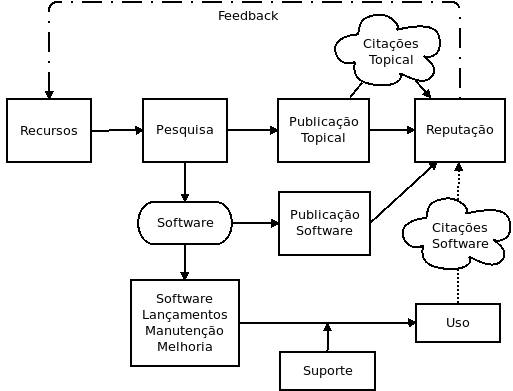
\includegraphics[scale=0.5]{imagens/scientific-reputation-diagram.png}
  \caption{A depiction of the reputation incentives in a mixed science and software academic practice \cite{howison2011scientific}}
  \label{scientific-reputation-diagram}
\end{figure}

%ecossistema de software acadêmico está inserido num contexto de competição

Diferentemente de outras tecnologias, software pode ser copiado e distriduído
essencialmente sem custo, abrindo portas sem precedentes em nível para
compartilhamento e inovação colaborativa \cite{howison2011scientific}, no
entando, estar em algum ponto no contexto de competição da economia de
reputação científica, em alguns pontos, como no mecanismo de crédito acadêmico
às produções ser potencialmente problemático para a colaboração e manutenção
\cite{howison2011scientific}.

No entanto tem se percebido que o ecossistema de software acadêmico tem perdido
oportunidade de colaboração visto que estão inseridos neste contexto ....
competição, muitos softwares utilizados em pesquisas não são mencionados pelos
seus autores causando impacto negativo em sua visibilidade, reconhecimento e
consequentemente ...  \cite{howison2016software}. Esta reflexão tem mostrado,
por exemplo, que muitos estudos em engenharia de software sofrem de
dificuldades de repetição \cite{tang2016worthiness}, e apontam problemas específicos
relacionados à manutenabilidade e a sustentabilidade técnica dos softwares
acadêmicos.

Este cenário, além de desacelerar o progresso geral da Ciência gerando
retrabalho, faz surgir questionamentos sobre as conclusões dessas pesquisas,
especialmente quando grande parte dos pesquisadores não sabem o quão confiável
seus softwares são. Junto com estas questões estão as questões de como
influenciar o ecossistema, incluindo questões de pontos de inflexão que levam
ao uso coalescente, bem como a intervenções políticas diretas incentivando o
uso de componentes específicos.

%%%%%%%%%%%%%%%%%%%%%%%%%%%%%%%%%%%%%%%%%%%%%%%%%%%%%%%%%%%%%%

%While some of these seem relatively unproblematic, such as commercial
%production in fields with immediately valuable applications, others appear
%problematic. In particular we highlighted the potentially pernicious
%implications of the academic credit production system for collaboration and
%maintenance 

%Adicionalmente as relacões entre os atores do ecosistema como um todo
%são de mútuo interesse (mutualismo):

%O relacionamento entre os atores em um ecossistema de software, por outro lado,
%são caracterizados pela alto espectro de relacionamentos simbioticos.

%Dependendo dos atores e suas atividades, dois atores podem ter benefícios
%mútuos (mutualismo), estar em competição direta (competition/antagonism),
%estarem não afetados (neutralism) ou um não afetado enquanto o outro é
%beneficiado (amensalism) ou prejudicado (parasitism) por seu relacionamento

%em pesquisas sobre análise de código, ferramentas de analise estatica tem
%recebido significante mais atencao que outras tecnicas, tecnicas com formal e
%bem definidos processos recebem mais atencao de pesquisa e escrutinio porque
%estudos irao avaliar seu processo e elementos, entretanto, isto nao
%necessariamente significa que tecnica é melhor; The survey concluded that 1)
%the adoption of static code analysis techniques in the industry is influenced
%by the software life cycle model, while software product type and company size
%doesn’t have an influence. 2) The amount of attention a static code analysis
%technique has received in research doesn’t necessarily influence its adoption
%in industry indicating a gap between research and industry 3) company size,
%product type, and life cycle model do influence professionals perception on
%benefits/limitations.  \cite{ilyas2016static}

\section{Sustentabilidade de software acadêmico}

O desenvolvimento de software sustentável tem sido identificado como um desafio
chave no campo da Ciência e da Engenharia Computacional, se sustentabilidade
não for levada em consideração em projetos de software, não importa qual o
domínio ou qual o propósito do software, perde-se a oportunidade de causar
mudanças positivas no planeta e na sociedade \cite{becker2014karlskrona}.

Sustentabilidade de software apesar de ser um conceito complexo e com mútiplas dimensões,
levando a debates profundos, possui um conceito geral bastante simples: refere-se à
capacidade de perdurar e de continuar sendo suportado ao longo do tempo, o que 
implica nas qualidades de longevidade e manunenabilidade do software
\cite{venters2014software}.

%Sustentabilidade de software tem sido um tema de intenso debate e inúmeras definições,
%frameworks, modelos, propostas de tornar sustentabilidade como um requerimento
%não-funcional de software, no entando em todos os em resumo uma conclusão tem sido
%geral e central, entre os frameworks, o contexto onde o software está inserido influencia na medição
%de sustentaabilidade \cite{venters2014software}. No entando, uma definição
%comum e compartilhada ainda não é realidade, não existe ainda uma definição
%clara do que significa sustentabilidade de software, e isto não pode ser
%subestimado. Entretando, esta falta de concenso, junto ao fato de que uma
%visão comum entre as propostas de frameworks para sustentabilidade é de que
%a definição e medição está intimamente relacionada ao contexto, ou domínio do
%problema \cite{venters2014software}, dessa forma uma boa estratégia de colaborar com esta grande figura é
%definir sustentabilidade em recortes distintos, como, sustentabildiade de
%software acadêmico de análise estática, por exemplo.

Software sustentável é aquele que continua a estar disponível no futuro, em
novas plataformas, atendendo continuamente às novas necessidades do ambiente
através de uma adequada evolução frente as condições em constante mudança
\cite{allen2017engineering}. Este conceito, no entando, ao ser aplicado ao
contexto de software acadêmico e artefatos digitais, mostra-nos um cenário
bastante preocupante, uma vez que, estudos recentes mostram que há uma tendêcia
ao decaimento de URLs ao longo do tempo, em publicações com produção de
artefatos digitais disponibilizados nestes endereços tem uma tendência a
tornarem-se indisponíveis ao longo dos anos \cite{wren2017use}.

Isto tem motivado iniciativas de tornar estes artefatos duráveis e disponíveis,
visando especialmente garantir a longevidade dos artefatos e proporcionar que
um segundo pesquisador receba todos os benefícios do trabalho duro do primeiro
pesquisador \cite{king1995replication},
o {\it Journal of the American Statistical Association (JASA)}, por
exemplo, tem insistido na necessiade de estar disponíveis código e dados ao
menos durante a revisão dos manuscritos \cite{baker2016scientists}, agências de
financiamento, como o {\it US National Science Foundation}, estão começando a
reconhecer produtos de pesquisa, como software, assim como fazem com as
publicações, tornando o software produzido em pesquisas cidadão de primeira
classe na Ciência \cite{allen2017engineering}.

Isto garante longevidade mas não implica em boa manutenibilidade, uma qualidade especialmente
importante aos projetos de software acadêmico, visto que sua qualidade tem sido questionada, onde a maioria dos cientistas autores
de software não sabe o quão confiável seu software é
\cite{merali2010computational}, muitos dos projetos de software acadêmico estão
em estado inicial de desenvolvimento \cite{marshall2013tools}, poucos foram
testados fora do contexto onde foram desenvolvidos \cite{portillo2012tools}.

\subsection{Problemas}

Não é difícil perceber que o ecossistema de software acadêmico sofre graves
problemas, percepção bastante similar ao fenômeno chamado de  desordem
caótica disfuncional ({\it ``dysfunctional chaotic churn''}), caracterizado
por:

\begin{quote}
Existência de muitos projetos, com poucos usuários, com
ciclos de vida curtos, que terminam em paralelo ao financiamento inicial,
comunidades desconectadas e paralelas, incompatibilidades entre projetos, e
tentativas aparentemente não coordenadas de ``reiniciar'' tudo ({\it re-boots})
\cite{howison2015understanding}.
\end{quote}

Este problema, apesar de ser apenas uma percepção, coincide com inúmeras
evidências a respeito de problemas com o desenvolvimento, reconhecimento e
sustentabilidade de software acadêmico \cite{allen2017engineering}.

%sabe-se que parte dos problemas são realmente fato, por exemplo,
%o {\it Dagstuhl Perspective Workshop}, evento organizado por um grupo de
%pesquisadores sêniores de renome internacional, realizado anualmente na
%universidade de Dagstuhl\footnote{\url{http://www.dagstuhl.de}} com o objetivo
%refletir sobre o estado da ciência da computação explorando tópicos novos e
%emergentes, em sua mais recente edição o workshop debateu sobre software

\subsubsection{Desenvolvimento}

O desenvolvimento de software acadêmico exige, muitas vezes, conhecimento
específico sobre o domínio do estudo sendo realizado,
por exemplo, entender como o DNA genômico
se transforma em cristais de proteína, ou estar familiarizado com os meandros
da dinâmica dos fluidos, ou saber como resolver 20 equações diferenciais
parciais simultâneas \cite{segal2008developing}.

Isto explica a grande participação dos cientistas no desenvolvimento de
software acadêmico, estudos tem mostrado que no reino unido entre todas as
áreas da ciência 56\% dos cientistas estão envolvidos no desenvolvimento de
software acadêmico \cite{hettrick2014uk}, outros estudos em grupos específicos mostram números ainda
maiores, na astronomia, por exemplo, 90\% dos cientistas desenvolvem software
acadêmico \cite{momcheva2015software}.

No entanto, a maior parte dos cientistas nunca tiveram treinamento algum sobre como escrever
software de forma eficiente, muitos não testam ou documentam os seus projetos de
software, faltam práticas básicas de desenvolvimento, como escrever código
legível, revisão de código, controle de versão, testes unitários, entre outros
\cite{wilson2017good}.

Isto tem ocasionado sérios erros computacionais em conclusões centrais da
literatura acadêmica, gerando retrabalho para retratar tais erros nas mais
diversas áreas da ciência \cite{merali2010computational}.
Dados são perdidos, análises levam mais tempo que o necessário e os
pesquisadores não conseguem a eficiência que poderiam ter ao trabalhar com
software acadêmicos \cite{wilson2017good}.
Causando um impacto negativo na visibilidade do software acadêmico e na
capacidade de ser encontrado e compartilhado \cite{howison2013incentives,
katz2014transitive}.

\subsubsection{Reconhecimento}

% visibilidade

Apesar do crescimento no uso de software e na consequente dependência entre
cientistas de todos os campos, tornando o software acadêmico parte integral da
prática científica, apesar do apelo da comunidade científica para que o
software acadêmico seja tratado como cidadão de primeira classe, estudos tem
mostrado que muitas pesquisas não mencionam sequer o uso de software acadêmico
em suas publicações mesmo tendo feito uso de tais artefatos
\cite{momcheva2015software} \cite{howison2016software}.

Isto tem prejudicado a visibilidade do software acadêmico causando impacto
negativo em seu ecossistema, um software invisível é frequentemente excluído de
revisões por pares, uma atividade que costuma contribuir para a qualidade geral
do trabalho publicado, além disso, o
impacto negativo na visibilidade do software acadêmico faz surgir uma
série de questionamentos sobre a sua qualidade e também sobre a
capacidade de ser encontrado, compartilhado e co-desenvolvido
\cite{howison2013incentives, katz2014transitive} \cite{howison2016software}.

Apesar de nem sempre ser possível, ou viável, ter tudo dentro de padrões
estritos, é preciso estar consciente das boas práticas ao produzir e utilizar
software acadêmico, tanto para melhorar a própria abordagem quanto para
revisar outros trabalhos \cite{wilson2014best}. Um software acadêmico em bom
funcionamento devem atingir não apenas os objetivos de entendimento e
transparencia, mas também os objetivos voltados para replicação
\cite{stodden2010reproducible}, seja logo após sua publicação, seja daqui a 10 ou 50 anos.

\subsubsection{Manutenibilidade}

% falar de manutenibilidade como um eixo dentro de sustentabilidade técnica

Manutenibilidade é uma característica de qualidade que indica o quão fácil é
realizar atividades de evolução e manutenção em software
\cite{kumar2012survey}, um aspecto importante aos pesquisadores interessados em
adaptar software acadêmico, algo muitas vezes necessário ao reproduzir
pesquisas anteriores \cite{peng2011reproducible}.

Estudos tem mostrado que grande parte das ferramentas de software criadas na
academia estão em estado inicial de desenvolvimento \cite{marshall2013tools} e
que apenas uma pequena porcentagem são testados fora do contexto onde foi
desenvolvido \cite{portillo2012tools}.

%A adoção e uso de software acadêmico está relacionado também à sua qualidade,
%portanto é importante medir e coletar sua qualidade de alguma forma, qualidade
%é um vasto assunto, um dos problemas comuns enfrentado pelos pesquisadores que
%desenvolvem tais projetos de software é a manutenibilidade \cite{prlic2012ten}.

A adoção e uso de software acadêmico está relacionado também à sua qualidade,
portanto é importante medir e coletar sua qualidade de alguma forma,
manutenibilidade apesar de ser um atributo de qualidade de software
inerentemente externa, pode ser medida através de
características de qualidade interna \cite{hashim1996software,
dagpinar2003predicting}, uma vez que grande parte dos engenheiros de software
assumem que uma boa estrutura interna resulta em boa qualidade externa
\cite{fenton2014software}.

No entanto é importante compreender os projetos de software acadêmico também em
termos de evolução e ciclo de vida, algo que pode influenciar enormemente as
medidas de qualidade medidas através de atributos internos do software, como
métricas de código fonte, por exemplo. 

%Iniciativas desta natureza resolvem o problema de disponibilidade destes
%artefatos mas ainda não garantem adequada evolução frente a contínua mudança
%do ambiente, apesar de sustentabilidade não implicar diretamente em qualidade,

%Tanto a ciência quanto a
%engenharia dependem de resultados incrementais para sua evolução. No terceiro
%compromisso, relacionado ao conceito {\it desenvolvimento}, o Dagstuhl
%Manifesto enfatiza a necessidade de medir a qualidade e a sustentabilidade dos
%softwares científicos, tanto a priori quanto a posteriori.

%Um estudo sobre ecossistema de software acadêmico percebeu através dos relatos
%de grande parte dos colaboradores participantes do estudo que os projetos de software
%acadêmicos desenvolvidos na própria academia 

%Olhar melhor os atributos de qualidade no artigo de Venters:
% https://openresearchsoftware.metajnl.com/articles/10.5334/jors.ao/
% We propose that software sustainability should be considered in a similar manner to the concept of dependability[16]; 
% a measure of a system’s availability, integrity, maintainability, reliability, and safety 
% where the attributes of dependability are defined as:
% Availability: readiness for correct service;
% Integrity: the absence of improper system alteration;
% Maintainability: undergo modifications and repairs;
% Reliability: continuity of correct service;
% Safety: the absence of catastrophic consequences on the user(s) and the environment.

%\begin{comment}
%
%We propose that software sustainability can be defined as ‘a measure of a systems extensibility, interoperability, maintainability, portability, reusability, scalability, and usability’ where the attributes are defined as:
%Extensibility: a measure of the software’s ability to be extended and the level of effort required to implement the extension;
%Interoperability: the effort required to couple software systems together.
%Maintainability: the effort required to locate and fix an error in operational software;
%Portability: the effort required to port software from one hardware platform or software environment to another;
%Reusability: the extent to which software can be reused in other applications;
%Scalability: the extent to which software can accommodate horizontal or vertical growth.
%Usability: the extent to which a product can be used by specified users to achieve specified goals with effectiveness, efficiency, and satisfaction in a specified context of use.
%If we accept that the concept of sustainability goes beyond the software artifact itself then other quality attributes such as efficiency may be appropriate candidates:
%Efficiency: the amount of computing resources and code required to execute a function.
%
%\end{comment}

\section{Ciclo de vida de software}
\label{sec:ciclo}

Engenheiros de software têm tradicionalmente considerado qualquer trabalho após
o primeiro lançamento de um software simplesmente como manutenção. Alguns
pesquisadores no entanto têm dividido este trabalho em atividades distintas, incluindo
adaptação, prevenção, correção, entre outras, mas sempre considerando manutenção
basicamente uniforme ao longo do tempo \cite{rajlich2000staged}.

Entretanto, alguns estudos têm demonstrado que esta visão, onde manutenção
ocupa um papel basicamente uniforme ao longo do tempo, não explica muito bem o
desenvolvimento de software na maior parte dos cenários e uma das abordagens
para explicar o fenômeno tem colocado a atividade de manutenção distribuída ao
longo do ciclo de vida do software \cite{rajlich2000staged}.

Este modelo de evolução do software em estágios, no entanto, foi avaliado e adaptado
ao contexto de software livre \cite{capiluppi2007adapting} e diante das
semelhanças com o software acadêmico, este modelo adaptado ao software livre serve ao propósito de ser
utilizado para
avaliar a evolução do software acadêmico. A Figura \ref{staged-model-foss-cycle}
apresenta o modelo de evolução adaptado ao software livre, adotado
neste estudo como aplicável também ao software acadêmico.

\begin{figure}[h]
  \center
  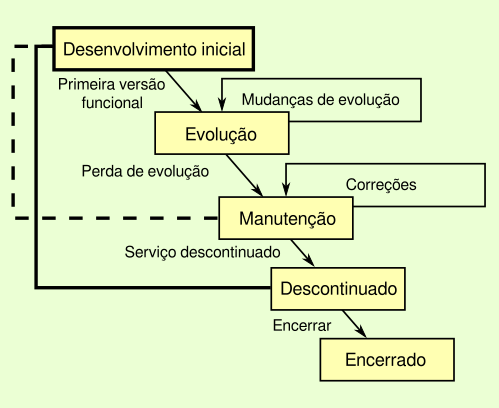
\includegraphics[scale=0.6]{imagens/staged-model-foss-cycle.png}
  \caption{O modelo de evolução {\it staged model} adaptado a software livre \cite{capiluppi2007adapting}.}
  \label{staged-model-foss-cycle}
\end{figure}

A primeira diferença observada é em relação a fase {\it Desenvolvimento inicial},
dependendo da definição de ``fase inicial'' muitos projetos de software livre
podem nunca ter saído desta fase, assim é também para o software acadêmico. Em respeito aos lançamentos,
em sistemas comerciais tradicionais eles devem ser completos, rodando e autorizado
pela empresa detentora, enquanto no mundo do software livre é comum
permitir acesso público ao código em repositórios de código fonte, seguindo
um modelo de ``versão permanente''.

A segunda diferença é relacionada à possibilidade de laços entre
as fases {\it Evolução} e {\it Manutenção}. Muitos projetos de software livre
possuem fases de congelamento na adição de novas funcionalidades ({\it freeze})
enquanto permanece numa fase de {\it Manutenção} até o descongelamento, voltando
a {\it Evolução}.

A terceira diferença está na comunidade de software livre,
novos times de desenvolvimento são formados ao longo do tempo
com a saída de desenvolvedores antigos e a entrada de novos.
E projetos em fase {\it Descontinuado} podem experimentar um renascimento
retornando ao período de {\it Evolução}.

Apesar das diferenças, os autores \citeonline{capiluppi2007adapting} demonstram em experimentos e
revisão de literatura que o modelo adaptado pode ser utilizado para
compreender evolução de software livre, e diante as similaridades entre software livre
e software acadêmico, este modelo poderá, consequentemente, ser também
utilizado para compreender a evolução e ciclo de vida do software acadêmico.

\section{Ciência e colaboração}

%Isto contradiz as boas práticas de qualquer projeto experimental ({\it
%laboratory
%notebooks}\footnote{\url{https://en.wikipedia.org/wiki/Lab_notebook}}, dados
%organizados, passos documentados, projeto estruturado para reprodutibilidade) e
%torna praticamente impossível utilizar o método mais comum e cientificamente
%produtivo de produzir conhecimento novo a partir de pesquisas anteriores, a
%replicação, ou seja, seguir os mesmos passos do autor original com
%objetivo de validar, melhorar ou estender seus dados e sua metodologia
%\cite{king1995replication, Stodden2010}.

%estas práticas permitem replicar descobertas anteriores seguindo
%o caminho do autor original,
%isto, segundo
%
% Replicability is not Reproducibility: Nor is it Good Science
%
% I want to challenge this view by separating
% the notion of reproducibility, a generally de-
% sirable property, from replicability, its poor
% cousin. I claim there are important differ-
% ences between the two. Reproducibility re-
% quires changes; replicability avoids them. Al-
% though reproducibility is desirable, I contend
% that the impoverished version, replicability,
% is one not worth having.
% ...
% In this paper, I have claimed that what many in the
% field are advocating is the replicability of published
% experiments. They argue that this meets the repro-
% ducibility requirement inherent to science. My claim
% is that replicability is a poor substitute for scientific
% reproducibility. There may be other good reasons for
% the collecting of software and scripts that are the ba-
% sis of the experimental results published in papers but
% scientific reproducibility is not one.
%
%The lack of replicability and reproducibility of scientific studies based on
%computational methods has lead to serious mistakes in published scientific
%findings, some of which have been discovered and publicized recently. Many
%strategies are currently pursued to improve the situation. This article reports the
%first conclusions from the ActivePapers project, whose goal is the development
%and application of a computational platform that allows the publication of
%computational research in a form that enables installation-free deployment,
%encourages reuse, and permits the full integration of datasets and software into
%the scientific record. The main finding is that these goals can be achieved with
%existing technology, but that there is no straightforward way to adapt legacy
%software to such a framework \cite{hinsen2014activepapers}
%
%
%% Ainda existem poucos estudos replicados \cite{kitchenham2015evidence}.

% Em resumo os dois manifestos, Dagstuhl e Karlskrona, exprimem o conceito de
% sustentabilidade necessários para este estudo, mas é importante citar que
% algumas iniciativas e outros manifestos também estão preocupados com questões
% similares, dentre os quais podemos destacar:
% 
%A ciência aberta e comunidades de pesquisa em software tem sido bastante ativas
%em criar manifestos visando chamadas para ação. Estes manifestos chamam para melhorar
%os softwares e os metadados de bibliografia para citação persistente destes softwares.
%Outros tópicos endereçados nestes manifestos incluem ênfase no acesso ao código fonte.

% Software Sustainability: The Modern Tower of Babel

%Somado a isto temos ainda o fato de que pesquisadores raramente publicam seus
%códigos, piorando ainda mais toda a situação, isto tem motivado a organização
%de conferências específicas para discutir os problemas dos softwares
%acadêmicos, como o RSE (Conference of Research Software Engineers)\footnote{
%\url{http://rse.ac.uk/conf2017}}, WSSSPE (Workshop on Sustainable Software for
%Science: Practice and Experiences)\footnote{
%\url{http://wssspe.researchcomputing.org.uk}} e o RESER (Workshop on
%Replication in Empirical Software Engineering Research)\footnote{
%\url{http://sequoia.cs.byu.edu/reser}}, e tem agregado discussões das
%comunidades de ciência aberta, reprodutibilidade e sustentabilidade de
%software.

%A ciência caminha sob a teoria e experimentação \cite{vardi2010science}. Não existe ciência fechada.

%Há uma explosão de dados abertos disponíveis on-line que é acessado e analisado
%através da criação de um novo software - gerando mais dados para analisar. Os
%softwares, ou seja, qualquer software que adquira, limpe, armazene, anote,
%transforme, filtre, gere (etc.) dados de pesquisa.

%\section{Seção sem nome ainda}

Estes são alguns problemas relacionados aos softwares acadêmicos, muitos são
resultado de baixos orçamentos, limitação de tempo e alta rotatividade entre os
grupos de pesquisa, outros são, possivelmente, ocasionados por questões
culturais \cite{niemeyer2017open}, como, por exemplo, a tímida adoção de
práticas da ciência aberta entre pesquisadores. Compreender os reais motivos
por trás destes problemas seria, naturalmente, o passo essencial para solucioná-los,
apesar disso, antes mesmo de resolver tais questões é
fundamental compreender os impactos que eles causam na comunidade de pesquisa.

Isto se torna ainda mais difícil visto que frequentemente os pesquisadores
deixam de publicar o código dos seus softwares acadêmicos argumentando que o
código é ``ruim'' e isto irá gerar julgamentos negativos ao pesquisador
\cite{allen2017engineering}.

Os compromissos expressados neste manifesto são agrupados em três conceitos gerais:
(i) garantir que softwares científicos sejam {\it citados} apropriadamente;
(ii) promover a {\it carreira} do engenheiro de software desenvolvedor de software científico; e
(iii) medir a qualidade e sustentabilidade do software científico durante e após o seu {\it desenvolvimento}.

um caminho apontado como solução é acreditar que software deve evoluir para plataformas compartilhadas,
com componentes reusáveis tanto quanto possível, tanto para usuário final, quanto
para produtores de componentes (papel) agregando peças particulares de software,
crença de que o software deve evoluir em direção a uma plataforma
compartilhada, com componentes que são reutilizados o mais amplamente possível,
já que os usuários finais e os produtores de componentes se agrupam em torno de
peças específicas de software.

Essa definição de sustentabilidade de software é encontrada em mais detalhes no
{\it Karlskrona Manifesto} \cite{becker2014karlskrona}, um documento que alerta
sobre os impactos que os sistemas e a tecnologia da informação causam no futuro
do planeta, convida praticantes e pesquisadores de software a refletir sobre
o tema sustentabilidade na área da ciência da computação.

\subsection{Reprodutibilidade}

Enquanto pesquisadores publicam artigos descrevendo e divulgando seus
resultados, é raro que façam o mesmo com toda a produção gerada durante a
pesquisa. A maioria dos componentes necessários para a reprodução dos
resultados de uma pesquisa -- por exemplo, códigos fonte e dados -- usualmente
permanecem não publicados. Esse problema fere um dos fundamentos
da ciência de que novas descobertas sejam reproduzidas antes de serem
consideradas parte da base de conhecimento \cite{Stodden2009}.

%Nesse sentido, \citeonline{Prlic2012} enfatizam que disponibilizar o código
%criado durante pesquisas não apenas aumenta o impacto como também se torna
%essencial para outros reproduzirem os resultados encontrados, citam ainda que
%manutenabilidade e disponibilidade do software após a publicação é o maior
%problema enfrentado pelos pesquisadores que desenvolvem tais softwares.
%
%A replicação desses estudos empíricos pode, e deve, ser realizado, de modo a
%averiguar a validade e aumentar o nível de confiança em seus resultados,
%replicação costuma ser citado como um importante meio para validar estudos
%empíricos e assim aumentar o nível de confiança em seus resultados
%\cite{Almqvist2006}. A reprodução dos resultados de pesquisas aumenta o impacto
%social das pesquisas e gera economia de tempo e dinheiro para os pesquisadores
%e para as instituições \cite{Nesta2010}.

Apesar da preocupação com a reprodutibilidade dos resultados de pesquisas de
forma independente \cite{Stodden2009} e aberta, esta área tem recebido ainda
pouca atenção da comunidade de pesquisa \cite{Nancy2015, Grand2010Open}. Em um
estudo recente, com 88 papers do MSR entre 2004-2011, evidenticou-se que apenas
62\% são replicaveis ou parcialmente replicaveis e que apenas 20\% dos estudos
disponibilizam suas ferramentas \cite{amann2015software}. Um estudo anterior
com 171 papers do MSR evidenciam que, entre outros problemas, a maioria não
disponibilizam publicamente as ferramentas e scripts, mesmo quando os autores
explicitamente afirmam que construíram algum \cite{robles2010replicating},
apenas 2 entre 154 estudos experimentais avaliados fornecem os dados e as
ferramentas necessárias para replicação e futuras pesquisas
\cite{barr2010shoulders}.

Reprodutibilidade ({\it reproducibility}) é a habilidade de replicar um experimento
ou estudo em sua totalidade a fim de confirmar suas hipóteses, seja pelo
autor ou por pesquisadores independentes. Esse conceito é um ponto
central do método científico e continua a receber bastante atenção ainda hoje,
como pode ser verificado em estudos recentes.

\citeonline{Stodden2009} preocupada com as barreiras legais para
disponibilidade de artefatos de pesquisa propõe o framework ``{\it Reproducible
Research Standard (RRS)}'', onde sugere formas de usar o licenciamento e as leis
de copyright da melhor forma para manter disponíveis os produtos gerados
durante pesquisas e assim viabilizar reprodutibilidade. \citeonline{Vitek2011}
em um estudo sobre reprodutibilidade e rigor científico destacam a importancia
de se disponibilizar qualquer material suplementar gerado durante uma pesquisa
de modo a possibilitar revisores verificarem e replicarem experimentos. Em
2012, um workshop intitulado ``{\it Reproducible Research: Tools and Strategies for
Scientific Computing}'' \cite{Stodden2012} discutiu, especificamente, iniciativas
e ferramentas voltadas a apoiar pesquisas reprodutíveis.
\citeonline{Krishnamurthi2015}, em um estudo sobre repetibilidade, chamam
atenção para o papel central que os artefatos de software possuem em pesquisas
de ciência da computação e questionam: "Onde está o software nas pesquisas
sobre linguagem de programação?". \citeonline{Stodden2015} demonstram o
projeto "ResearchCompendia.org", uma infraestrtura para reprodutibilidade e
colaboração em ciência computacional. Além destes e tantos outros estudos em
\cite{GithubReproducibilityGuide} é possível acessar um guia sobre como
desenvolver pesquisas cientíticas de forma que promovam a reprodutibilidade.

Apesar do termo reprodutibilidade ser relativamente concensual entre as várias
áreas da ciência, existem alguns termos relacionados com uma certa diferença
de significado, diante disto, e preocupado em criar uma linguagem comum entre
os pesquisadores, \citeonline{Feitelson2015} propôs as seguintes definições:

\begin{description}

  \item[Repetição (repetition)]
  Refazer exatamente o que outra pessoa fez usando os artefatos originais.

  \item[Replicação (replication)]
  Replicar com precisão exatamente o que outra pessoa fez, recriando os
  artefatos.

  \item[Variação (variation)]
  Repetir ou replicar exatamente o que a outra pessoa fez, mas com alguma
  modificação controlada nos parâmetros.

  \item[Reprodução (reproduction)]
  Recriar o espírito do que outra pessoa fez, usando seus próprios artefatos.

  \item[Corroboração (corroboration)]
  Obter os mesmos resultados de outra pessoa, usando outros meios e
  procedimentos experimentais.

\end{description}

É conhecido que a ciência precisa de reprodutibilidade e corroboração para
realmente fazer progressos, mas a prática de forma abrangente ainda é um
obstáculo. Diante disso \citeonline{Peng2011} sugere adotar soluções
intermediárias, repetição, replicação, variação, e desta forma já teríamos uma
grande melhoria sobre a situação atual onde muitos estudos em engenharia de
software sofrem de dificuldades de repetição \cite{Tang2016} e,
consequentemente, poucos estudos replicando pesquisas da área são encontrados
\cite{da2011replication}.

Mesmo sabendo que todo artefato tem impacto na reprodutibilidade
\cite{gonzalez2012reproducibility}, uma barreira comum para tal prática, e
consequentemente para repetição, replicação e variação é a indisponibilidade do
código fonte. Toda pesquisa que possua qualquer processo computadorizado deve
publicar seus códigos, eles precisam estar disponíveis, mesmo que os dados
correspondentes não estejam, o código deve estar. De acordo com o espectro de
reprodutibilidade (Figura \ref{reproducibility-spectrum}), a disponibilidade de
código é o requisito mínimo e é o primeiro passo para possibilitar validação e
confirmação dos resultados.

\begin{figure}[h]
  \center
  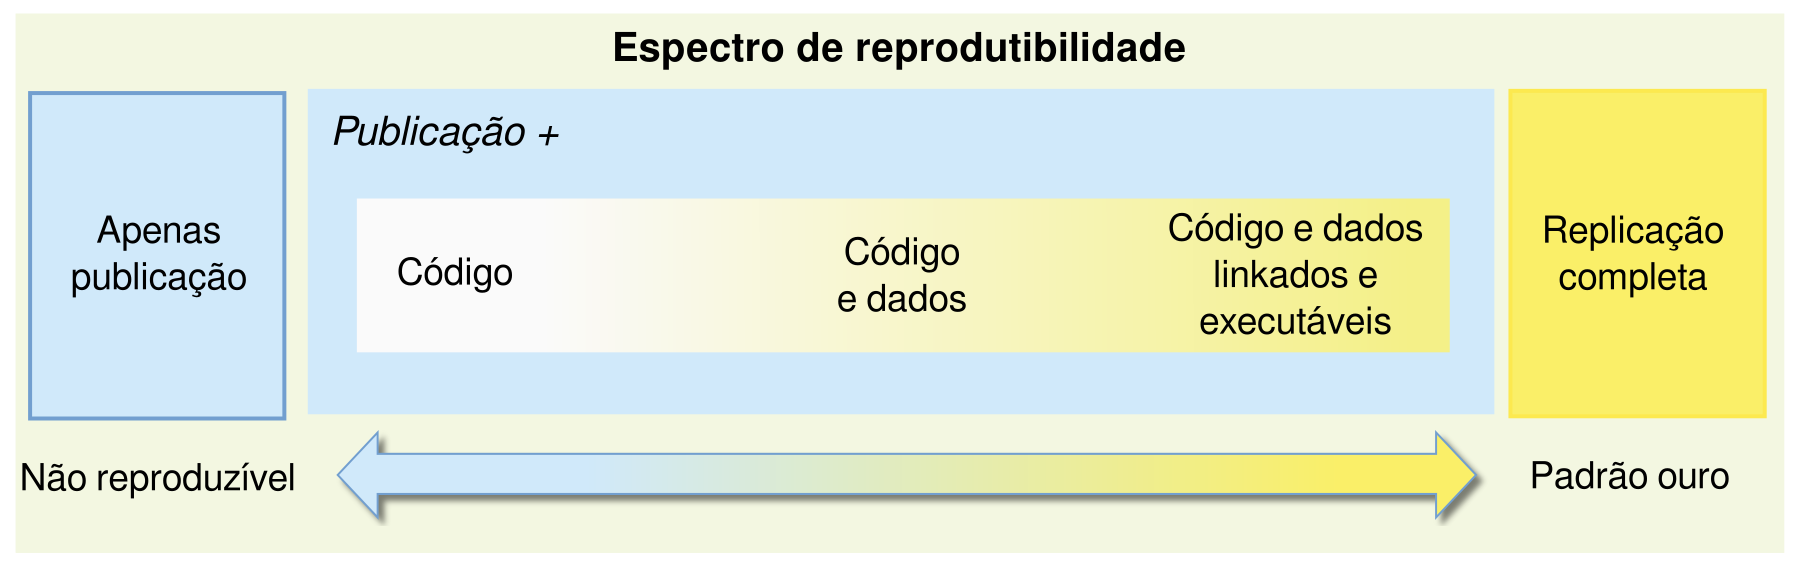
\includegraphics[scale=0.35]{imagens/reproducibility-spectrum-ptbr.png}
  \caption{Espectro de reprodutibilidade \cite{Peng2011}}
  \label{reproducibility-spectrum}
\end{figure}

Apesar das pesquisas reproduzíveis ({\it RR - Reproducible Research}) não
resolverem todos os problemas de validade experimental dos estudos em
engenharia de software, elas ao menos garantem que dados e métodos de análise
estejam disponíveis para inspeção e que os resultados possam ser derivados,
facilitando revisão logo que a publicação acontece. Além disso, é um recurso
valoroso para pesquisadores iniciantes, pesquisas reproduzíveis melhoram o
impacto do próprio estudo, por exemplo, artigos de computação que não
disponibilizam pubicamente dados e códigos possuem menos chances de serem
citados \cite{madeyski2017would}.

\subsection{Ciência aberta}

Ciência Aberta é um movimento que tem por objetivo tornar a pesquisa
científica, seus dados e sua disseminação acessíveis à todos os interessados,
sejam amadores ou profissionais \cite{WikipediaOpenScience}. Sua principal
motivação está em possibilitar a reprodução dos resultados de pesquisas e em
garantir transparência das metodologias utilizadas, isto aumenta o impacto
social das pesquisas e gera economia de tempo e dinheiro para os pesquisadores
e para as instituições \cite{Nesta2010}.

Este movimento é guiado por princípios básicos de transparência, acessibilidade
e reusabilidade universais, disseminadas via ferramentas online, ele é dividido
em quatro grandes áreas: (1) Open Access, (2) Open Data, (3) Open Source e (4)
Open Reproducible Research. Dentre elas destaca-se a Open Reproducible Research
por preocupar-se com a reprodutibilidade dos resultados de pesquisas de forma
independente \cite{Stodden2009} e aberta, no entanto, esta área tem recebido
ainda pouca atenção da comunidade de pesquisa \cite{Nancy2015}
\cite{Grand2010Open} apesar do aumento geral do interesse pelas práticas da
Ciência Aberta \cite{Grand2010}.

%Over the past fifteen years the scholarly communications agenda
%has progressed gradually. Currently we are experiencing a strong
%tendency among all research stakeholders to engage with the
%practice of OS. Lately, research funders require the sharing not
%only of the research results they have funded, but also of the
%procedures and data that are being generated during the research
%conduct. Researchers, on the other side, are keen on observing
%their research results being used for the improvement of the
%society and are forced by their funders to demonstrate the impact
%of their research. At the same time, higher academic institutions
%aim to join the OS agenda as well, since they see the opportunity
%of great economic benefits and savings. While OS is the possible
%answer to all these factors, the stakeholders’ inability to
%understand the requirements for the application of OS can be a
%suspensory factor for the OS implementation and evolution.
%The aim of the FOSTER project is to advance the stakeholders'
%knowledge on the usefulness of OS and explain the technicalities,
%strategies and best practices using which OS can be applied. As an
%attempt to educate the largest number of researchers possible,
%FOSTER has created an e-leanring portal, which contains quality
%assured information relating to the topic and it is open to everyone
%in the world. The platform contains two types of information:
%learning material and online courses. The classification of these
%two types is supported by an OS taxonomy, where related terms
%are applied both in the portal's material and also in the courses.
%With the use of the taxonomy, users are in the position to
%understand the OS domain and the concepts around it.
%The main goal of the FOSTER project, which is mainly achieved
%through the portal functionalities, is not only to educate the
%research stakeholders on OS, but also to build a community of
%researchers, librarians, software developers, funders and research
%administrators who are interested in OS in order to advance the
%way research is being conducted and shared. In addition, FOSTER
%attempts to provide tools to this community, such as re-usable
%content for training and a platform for blended learning and e-
%learning courses that the community could run. This OS
%advancement is essential for the research promotion and,
%consequently, for the benefit of the society as a whole
%\cite{Nancy2015}.
%
%Open Science may be practised both
%for philosophical and pragmatic reasons. As the
%resources produced by open projects are
%potentially accessible to public audiences, Open
%Science offers both a novel medium for public
%access and involvement in the process of science
%and an innovative method for real-time science
%communication. Does such direct access clear
%the stream of communication or muddy the
%waters with unfocussed, unclear and unvetted
%comment? This paper suggests that adopting an
%Open Science approach allows the capture of an
%authentic and clear record of research.
%However, researchers acknowledge this involves
%opening their work up to a different type of
%scrutiny \cite{Grand2010}.
%
%Open Science is an emerging approach to the conduct of science, technology and engineering
%projects, in which information about the whole of an ongoing investigation is made available
%on and through the Internet. Adopting an Open Science approach means the audience for the
%research can extend beyond the researchers involved to other researchers and to members of
%the public. Thus, Open Science has implications for engineering research, practice,
%publishing and public engagement with engineering. This paper reviews the history and
%evolution of the Open Science movement, includes some reflections on the related areas of
%Open Access, peer-review and public engagement with science and engineering and discusses
%data gathered from interviews. The analysis suggests that interviewees have concerns about
%issues such as precedence and protection of original work and the time needed to integrate
%open science practices into daily work. Successfully working in such collaborations is likely
%to require not only common practical tools but also the development of shared language and
%understanding between researchers and members of the public. Interviewees recognise the
%value of Open Science in collaborative research and its innovative facility to sustain direct
%public access to research outputs. It also has the potential to allow members of the public to
%make real practical contributions to research \cite{Grand2010Open}.
%
%This white paper was written as a contribution to the “Imagining
%Tomorrow’s University: Rethinking scholarship, education, and institu-
%tions for an open, networked era” workshop, a joint NIH/NSF-funded
%event held 8–9 March 2017 in Rosemont, IL. In this paper, I present an
%overview of what I consider open science, its importance, and how it
%plays a role in my research agenda. I also discuss challenges faced in
%pursuing research openness, and recommend changes to university
%leaders to address these barriers \cite{niemeyer2017open}.
%
%Open to All?  Case studies of openness in research
%Since the early 1990s, the open access movement has promoted the concept of openness in relation
%to scientific research. Focusing initially upon the records of science in the form of the text of articles
%in scholarly journals, interest has broadened in the last decade to include a much wider range of
%materials produced by researchers. At the same time, concepts of openness and access have also
%developed to include various kinds of use, by machines as well as humans.
%Academic bodies, including funders and groups of researchers, have set out statements in support
%of various levels of openness in research. Such statements often focus upon two key dimensions:
%what is made open, and how; and to whom is it made open, and under what conditions? This study
%set out to consider the practice of six research groups from a range of disciplines in order to better
%understand how principles of openness are translated into practice \cite{Nesta2010}.

\subsection{Ciberinfraestrutura}

A visão da ciberinfraestrutura, expressada no "Relatório Atkins" e instanciada
para o ecossistema de software científico na NSF chamada de Infraestrutura de
Software para Inovação Sustentada (NSF SI2),

Os softwares vem não apenas atuando no avanço da ciência, mas atuando com uma
eficiência crescente ao longo do tempo (Atkins 2003). A chave para isso é a
crença de que o software deve evoluir em direção a uma plataforma
compartilhada, com componentes que são reutilizados o mais amplamente possível,
já que os usuários finais e os produtores de componentes se agrupam em torno de
peças específicas de software.

a literatura sobre plataformas de software fora da ciencia tem chamado isso de
'coring' e 'tipping' (Gawer and Cusumano 2008),
onde uma comunidade descobre sua funcionalidade compartilhada e se agrupa
em pacotes que fornecem, levando ao uso eficiente de recursos através de
economias de escala.

coring também resulta em um aumento do uso sobreposto que facilita mais

Isto também resulta em um aumento do uso sobreposto que facilita mais
transparência na ciência, levando a uma maior qualidade e correctude (correctness), à medida
que mais olhos e esforços são direcionados para os mesmos códigos que são
sustentados e evoluem em longos períodos de utilidade científica.

coring em direção às plataformas pode ser contrastado com o seu oposto, muitas
vezes percebido por informantes: churn caótico disfuncional, com muitos
projetos com poucos usuários, cada um tendo vidas curtas que terminam com o
financiamento de concessão inicial, comunidades desconectadas e paralelas,
incompatibilidades teimosamente imutáveis e periódicas e tentativas
aparentemente não coordenadas de "reiniciar". Subjacente a isso é uma
preocupação que as oportunidades são perdidas e que o progresso da ciência é
abrandado (por exemplo, Stewart, Almes e Wheeler 2010).

%%%%%%%%%%%%%%%%%

%chape para isto é acreditar que software deve evoluir para plataformas compartilhadas,
%com componentes reusáveis tanto quanto possível, tanto para usuário final, quanto
%para produtores de componentes (papel) agregando peças particulares de software

% fez exatamente o que pensei, vou ler para usar a metodologia "adaptada"
%In addition to these motivation studies, scientists have recently embarked on the issue of
%software use and impact. A study in 2013 has found that scientists tend to choose software
%that is widely used by others in their community and prefer software that is free for
%academic use (Huang et al. 2013). Studies on the scientific software ecosystem have
%suggested that the use of scientific software is influenced by its visibility, availability,
%sustainability, reproducibility, and citation (Howison and Herbsleb 2014; Howison et al.
%2015; Huang et al. 2013). Studies also have suggested that software developers are
%interested to know the use and impact of their software because ‘‘software use matters to
%them for funding purposes’’ (Howison et al. 2015; Trainer et al. 2015, p. 428).
%Recent studies on data impact have led to the discussions on software citation and
%evaluation, as a parallel can be drawn between software and data in scientific literature
%(Piwowar et al. 2011; Howison and Bullard 2016). It is suggested that the numbers of
%mentions and citations in literature can be used to measure the impact of software (Huang
%et al. 2013; Pan et al. 2015). Yet, it is argued that ‘‘the practices of citation to software vary
%considerably from field to field and appear to miss significant software’’ (Howison et al.
%2015, p. 478). One study examining the use of software in scientific articles in biology has
%found that more than half of the software mentions did not include references (Howison
%and Bullard 2016). Thus, it validates the need to use alternative metrics in addition to
%citations when assessing software impact, such as the numbers of downloads, registered
%users, subscribers, user reviews, and artifacts inserted in literature (Howison et al. 2015).

Assim, surge um conjunto de ações que podem ser tomadas pelos diferentes atores
em direção à garantir sustentabilidade nos projetos de software, ações para
praticantes de software, pesquisadores, associações profissionais, educadores,
cientes e usuários.

Inevitavelmente alguns softwares irão continuar sendo úteis após o primeiro
release, alguns terão algums gerações de melhorias, outros serão usados na sua
versão original sem atualização ou manutenção, e alguns outros irão ser
lançados e nunca utilizados. Isto é perfeitamente natural, a comunidade ao
redor do software irá decidir qual é o melhor caminho a se tomar num processo
evolutivo \cite{weiner2009astronomical}.

lugar, em algum momento. Uma utilidade óbvia para qualquer um destes softwares
é para aqueles que desejam replicar as pesquisas em que foram criados, seja com
o simples objetivo de validar as conclusões, seja com interesse de estender e
colaborar com a pesquisa original.

\subsection{Pesquisas reproduzíveis}

% Software Carpentry: lessons learned [version 2; referees: 3 approved]
%
% iniciativa voltada a melhorar as habilidades com computação entre os
% pesquisadores de diversas áreas, ajudando a melhorar os resultados,
% facilitar reprodutiblidade, acesso a dados, codigos, etc... reducao de custos
% melhoria de qualidade, etc... faz workshops, eventos, treinamentos, ao longo
% dos varios anos de existencia, ...
%
% Since its start in 1998, Software Carpentry has evolved from a week-long
% training course at the US national laboratories into a worldwide volunteer effort
% to improve researchers' computing skills. This paper explains what we have
% learned along the way, the challenges we now face, and our plans for the
% future.


% (6) A systematic literature review of software product line management tools \cite{pereira2015systematic}
%
% (???)
%
% (7) Software configuration management tools \cite{chan1997software}
%
% (???)

\subsection{Artigos executáveis}

...

\subsection{Software como cidadão de primeira classe na ciência}

JOSS, Papers executáveis, pesquisas reproduzíveis, etc, dar credibiidade ao
pesquisador cientista desenvolvedor de software ... papel do software na
reprodutibilidade, etc...

%A situação com software é amplamente análoga (mas não identica) ao de dados
%das publicações; de fato, todo dado é processado por softwares de alguma forma
%(Borgman et al., 2012).

%\item The GeoScience paper of the future initiative \cite{OntoSoft2016}\footnote{\url{http://www.scientificpaperofthefuture.org/gpf/what-is-a-gpf}}
%Possui um conjunto de requerimentos para softwares serem incluidos em
%papers.  Focando mais no paper em sí do que no software.

%Linked Open Science—Communicating, Sharing and Evaluating
%Data, Methods and Results for Executable Papers.
%Linked Open Science is an approach to solve challenges of an executable paper. It is a combination of four “silver
%bullets”: 1) publication of scientific data, metadata, results, and provenance information using Linked Data principles,
%2) open source and web-based environments for executing, validating and exploring research, 3) Cloud Computing
%for efficient and distributed computing, and 4) Creative Commons for the legal infrastructure. We will use a realistic
%scientific research setting related to research on deforestation of the Brazilian Amazon rainforest to provide scenarios
%to illustrate the application of Linked Open Science \cite{Kauppinen2011}.

%Diversas maneiras de inventivar citação formal entre artefatos digitais,
%software por exemplo, tem surgido, dentre elas uma iniciativa interessante
%é o Journal of Open Source Software (JOSS) é um livre a open-access jornal para
%publicação de artigos descrevendo software acadêmico. Ele tem dois objetivos
%principais, melhorar a qualidade dos softwares submetidos e prover mecanismos
%para pesquisadores desenvolvedores de software acadêmico receber crédito pelos
%seus softwares. Enquanto pensado para trabalhar dentro do atual sistema de
%mérito da ciência, JOSS visa a escassez de recompensas para contribuições
%importantes para a ciência realizadas em forma de software. JOSS publica
%artigos que encapsulam sabedoria contida no software ele mesmo, e seu rigoroso
%revisão em pares mirado nos componentes do software: funcionalidade,
%documentação, testes, integração contínua, e a licença. Um artigo JOSS contém
%um resumo descrevendo o objetivo e funcionalidades do software, referencias, e
%um link para o software archive.  O artigo é um ponto de entrada para
%submissçao que engloba o conjunto completo de artefatos de software. Artigos
%aceitos no JOSS recebem um digital object identifier (DOI), te seus metadados
%depositados no Crossref, e o artigo pode começar a colecionar citações e ser
%indexados em serviços como Google Scholar e outros. No seu primeiro ano,
%iniciado em Maio de 2016, JOSS publicou 111 artigos, com mais de 40 artigos
%adicionais sob revisão \cite{smith2017journal}.

%\item UK RSE \cite{ukrse2013}\footnote{\url{http://rse.ac.uk/who}}
%Conscientização sobre a importância e o papel do {\it Research Software
%Engineer} através de comunicação e suporta institucional.

%FORCE11 Software Citation principles \cite{smith2016software}\footnote{\url{https://www.force11.org/software-citation-principles}}
%Enfatiza persistencia e claridade e diz que ``Software deve ser considerado
%um produto legítimo de pesquisas e devem ser possível de serem citados''.

%Reproducibility verification is essential to the practice of the scientific method.
%Researchers report their findings, which are strengthened as other independent groups
%in the scientific community share similar outcomes. In the many scientific fields
%where software has become a fundamental tool for capturing and analyzing data, this
%requirement of reproducibility implies that reliable and comprehensive software platforms
%and tools should be made available to the scientific community. The tools will empower
%them and the public to verify, through practice, the reproducibility of observations that
%are reported in the scientific literature. Medical image analysis is one of the fields in
%which the use of computational resources, both software and hardware, are an essential
%platform for performing experimental work. In this arena, the introduction of the Insight
%Toolkit (ITK) in 1999 has transformed the field and facilitates its progress by accelerating
%the rate at which algorithmic implementations are developed, tested, disseminated and
%improved. By building on the efficiency and quality of open source methodologies, ITK has
%provided the medical image community with an effective platform on which to build a daily
%workflow that incorporates the true scientific practices of reproducibility verification. This
%article describes the multiple tools, methodologies, and practices that the ITK community
%has adopted, refined, and followed during the past decade, in order to become one of the
%research communities with the most modern reproducibility verification infrastructure. For
%example, 207 contributors have created over 2400 unit tests that provide over 84% code
%line test coverage. The Insight Journal, an open publication journal associated with the
%toolkit, has seen over 360,000 publication downloads. The median normalized closeness
%centrality, a measure of knowledge flow, resulting from the distributed peer code review
%system was high, 0.46 \cite{McCormick2014}.

%Among empirical software engineering studies, those based on data re-
%trieved from development repositories (such as those of source code management,
%issue tracking or communication systems) are specially suitable for reproduction.
%However their reproducibility status can vary a lot, from easy to almost impossible
%to reproduce. This paper explores which elements can be considered to characterize
%the reproducibility of a study in this area, and how they can be analyzed to better
%understand the type of reproduction studies they enable or obstruct. One of the
%main results of this exploration is the need of a systematic approach to asses the
%reproducibility of a study, due to the complexity of the processes usually involved,
%and the many details to be taken into account. To address this need, a methodology
%for assessing the reproducibility of studies is also presented and discussed, as a tool to
%help to raise awareness about research reproducibility in this field. The application
%of the methodology in practice has shown how, even for papers aimed to be
%reproducible, a systematic analysis raises important aspects that render reproduction
%difficult or impossible. We also show how, by identifying elements and attributes
%related to reproducibility, it can be better understood which kind of reproduction
%can be done for a specific study, given the description of datasets, methodologies and
%parameters it uses \cite{gonzalez2012reproducibility}.

%Science rests on peer review and the wide-spread dissemination of
%knowledge. Software engineering research will advance further and
%faster if the sharing of data and tools were easier and more wide-
%spread. Pragmatic concerns hinder the realization of this ideal: the
%time and effort required and the risk of being scooped. We examine
%the costs and benefits of facilitating sharing in our field in an effort
%to help the community understand what problems exist and find
%a solution. We examine how other fields, such as medicine and
%physics, handle sharing, describe the value of sharing for replication
%and innovation, and address practical concerns such as standards
%and warehousing. To launch what we hope will become an ongoing
%discussion of solutions in our community, we present some ways
%forward that mitigate the risk of sharing — partial sharing, registry,
%escrow, and market \cite{barr2010shoulders}.

%At various machine learning conferences, at
%various times, there have been discussions
%arising from the inability to replicate the
%experimental results published in a paper.
%There seems to be a wide spread view that we
%need to do something to address this prob-
%lem, as it is essential to the advancement
%of our field. The most compelling argument
%would seem to be that reproducibility of ex-
%perimental results is the hallmark of science.
%Therefore, given that most of us regard ma-
%chine learning as a scientific discipline, being
%able to replicate experiments is paramount.
%I want to challenge this view by separating
%the notion of reproducibility, a generally de-
%sirable property, from replicability, its poor
%cousin. I claim there are important differ-
%ences between the two. Reproducibility re-
%quires changes; replicability avoids them. Al-
%though reproducibility is desirable, I contend
%that the impoverished version, replicability,
%is one not worth having \cite{drummond2009replicability}.

%Abstract—This paper is the result of reviewing all papers
%published in the proceedings of the former International
%Workshop on Mining Software Repositories (MSR) (2004-2006)
%and now Working Conference on MSR (2007-2009). We have
%analyzed the papers that contained any experimental analysis
%of software projects for their potentiality of being replicated.
%In this regard, three main issues have been addressed: i) the
%public availability of the data used as case study, ii) the public
%availability of the processed dataset used by researchers and iii)
%the public availability of the tools and scripts. A total number of
%171 papers have been analyzed from the six workshops/working
%conferences up to date. Results show that MSR authors use
%in general publicly available data sources, mainly from free
%software repositories, but that the amount of publicly available
%processed datasets is very low. Regarding tools and scripts, for
%a majority of papers we have not been able to find any tool,
%even for papers where the authors explicitly state that they have
%built one. Lessons learned from the experience of reviewing the
%whole MSR literature and some potential solutions to lower the
%barriers of replicability are finally presented and discussed
%\cite{robles2010replicating}.

%A survey of controlled experiments in software engineering
%Among
%the 20 replications, five can be considered as close replica-
%tions in the terminology of Lindsay and Ehrenberg [31], i.e.,
%one attempts to retain, as much as is possible, most of the
%known conditions of the original experiment.

%Replication of empirical studies in software engineering: Preliminary findings from a systematic mapping study
%The number of replications grew in the last few years, but the
%absolute number of replications is still very small, in particular
%considering the breadth of topics in software engineering. Incentive
%to perform external replications and better standards to report
%empirical studies and their replications are still needed.

%Um fator em favor da aceitação dos conceitos da EBSE tem sido a crescente
%reconhecimento que os resultados de estudos empíricos individuais são frequentemente
%inconclusivos, e estes tipo de estudos são difícels de replicar com sucesso
%\cite{sjoberg2005survey}.

%\item Reproducibility manifesto \cite{Barba2012}\footnote{\url{http://lorenabarba.com/gallery/reproducibility-pi-manifesto}}
%Inclui termos para fazer softwares reusáveis por outros. Foco em
%reprodutibilidade, deixando sustentabilidade de software fora de questão.

%%%%%%%%%%%%%%%%%

Apesar do reconhecimento de vários destes problemas nas mais diversas
áreas da ciência, ainda não sabe-se como o ecossistema de software
acadêmico de análise estática se posiciona neste cenário.

